\chapter{Sonar Simulation}

\epigraph{If you cause your ship to stop, and place the head of a long tube in
the water and place the outer extremity\\ in your ear, you will hear ships at a
great distance from you.}{\textit{Leonardo Da Vinci}, 1490}


The ideia behind simulation is to have a flexible environment where the system
(e.g. sonar, reconstruction model) can be tested on a variety of conditions
and the ground truth is well known. It is a mature and wide spread
mechanism for development of new sonar technologies \cite{Etter2013}.

Opening this chapter, it will be presented physical foundations behind sonars,
and its existing technologies and models. Next describing the envisioned
environmental properties, and ending  with  a more detailed view of the
simulation technique used.

\section{Sonar}

Throughout this thesis only one type of sonar is considered, the mechanical
imaging active sonar\ref{ss:avaible_models}. Sonars have a common underlying
principle of operation, but vary greatly on aplication and hardware constituition.

Sonars are, in some sense, the acoustic analog of a camera. They use sound,
instead of light, to capture information about the environment. So, to better
undersand \textit{how} they operate and \textit{what} are they used for, it is
important to have a clear concept of sound.

\subsection{Physics of Sound}

The phenomenon that humans percieve as sound is a pressure wave that amplitude
excess the mean pressure of the medium \cite{FEYNMAN}. It can me referred to as
\textit{compressional} or \textit{longitudinal} waves, contrasting with
\textit{transversal waves}. The difference between these two kinds of waves
relies on the direction of the movement of the particles, being parallel or
perpendicular to the propagation of the wave, respectively\cite{BRUNEAU}.

On the particular, but usefull, conditions of low energy
phenomena\cite{Lefebvre} (with some other suitable requirements\footnote{A
perfect simple fluid in an initial state of stationary homogeneous equilibrium})
the pressure pertubation wave can be described as the \textit{D'Alembert
equation}:
 
\begin{equation}\label{eq:lambert}
\nabla^2 \Phi - \frac{1}{c^2_0}\frac{\partial^2}{\partial t^2} \Phi = 0
\end{equation}

Where $\Phi$ is the velocity potencial, a scalar field that helps describing the
sound propagation. Its relation to sound pressure is:

\[ p =  -\rho \frac{\partial}{\partial t}\Phi \]

Which can be directly described as:

\begin{equation} \label{eq:wave}
\nabla^2 p - \frac{1}{c^2_0}\frac{\partial^2}{\partial t^2} p = 0
\end{equation} 
 
Where $p$ is the pressure deviation from the mediums, $\rho$ the density, $c_0$
is the local sound speed and $\nabla^2$ stands for the Laplace operator. These equations are
only valid in free space (no source), but discrete variations of the medium are
treated as boundary conditions, giving origin to reflection and refraction.

Besides pressure, sound has another important derived property: intensity. Much
like the case of electromagnetic waves, sound intensity (or acoustic intensity)
measures the mean value of the sound energy flux (i.e. energy rate
per area):

\begin{equation}\label{eq:intensity_mean}
\vec{I} = \overline{p\vec{v}}
\end{equation}

Where $\vec{I}$ represents the \textit{acoustic intensity} vector, $\vec{v}$ the
\textit{acoustic velocity} (i.e. the velocity of a particle in the medium) and the
overline the mean over some time period. The \textit{acoustic velocity} can also
be derived from the velocity potencial $\Phi$ as:

\[ \vec{v} = \nabla \Phi\]

When considering a wave far from its source, solutions to the equation
\ref{eq:wave} give rise to a \textit{plane wave}( where the coherent wave front
propagate in a plane). It makes clear the relationship between $\vec{v}$ and
$p$:

\[ \vec{v} = \frac{p}{\rho c_0} \vec{n_0} \]

Where $\vec{n_0}$ is the unit normal vector to the wavefront. Pluging it back to
equation \ref{eq:intensity_mean}:

\begin{equation}\label{eq:intensity_pressure}
\vec{I} = \tfrac{1}{\rho c_0} \overline{p^2} \vec{n_0}
\end{equation}

This equation shows the proportionality between the \textit{acoustic
intensity} and the mean squared of the pressure. The inverse of the
proportionality constant $\rho c_0$ is called the \textit{characteristic
impendace} because it measures the degree of ``resistense to propagation'' of
the medium.

%By means of the same reasoning about the physical properties

 %(perpendicular to the direction of propagation)

Because the acoustic intensity (and related quantities) varies orders of
magnitude while propagating, it is commom to quantify it on a logarithmic scale,
specifically \textit{decibels} (dB)\cite{LURTON}:

\begin{equation}\label{eq:dB}
I_{dB} = 10~\log_{10}\left(\frac{I}{I_0}\right)
\end{equation} 

Here $I_{dB}$ is the intensity measured in \textit{decibels}, $I$ the intensity
value and $I_0$ a reference intensity values, usually defined somewhere near the
source. In the case of reflected/refracted wave, $I_0$ may also refere to
the intensity of the incoming wave. A direct relation between the magnitude of
intensity and pressure is found by applying equation \ref{eq:intensity_pressure}
on equation\ref{eq:dB}:

\begin{equation}\label{eq:dB}
I_{dB} = 20~\log_{10}\left(\frac{p_{\text{rms}}}{p_0}\right)
\end{equation}

Where $p_{\text{rms}}$ is the \textit{rms} (Root mean squared) value of the
wave's pressure ({\small $\sqrt{\text{\tiny \(\overline{p^2}\)}}$}) and $p_0$ is
a pressure value of reference, for underwater acoustics this value is the
microPascal (\(p_0 = 1~\mu\text{Pa} \))\cite{LURTON}.


\subsection{Sonar Principle of Operation}

The name Sonar (\textit{\underline{So}und \underline{N}avigation \underline{A}nd
\underline{R}anging}) was originally conceived for the tecnique that uses
acoustic waves on water for navigation, communication and detection, but
nowadays it is also used for the equipament that generate/receive these
sound waves.

The history is considered to have started on the year of 1490 through the
statemnt of Leonardo Da Vinci contained on the epigraph at the begining of this
chapter\cite{fahy1998fundamentals}. But that was birth of \textit{passive
sonar}'s technology, where the objetive is to listen (receive and process sound
waves) the noise from ships, animals and other objects in an attempt detect and
reconize its origin.

\subsubsection{Active Sonar}

The concept of an \textit{active sonar}, one that emits a sound wave and detects
its return (as in figure \ref{fig:sonar_principle}), is much more recent. The
loss of the \textit{HMS Titanic} to a collision with an iceberg during its first
voyage on April 15 of 1912 \cite{histsonar} fostered the development of a sonar
to detect objects kilometers away. Also, during World War I,
Allied shipping losses to U-boat attacks further stimulated advances on tecniques for
unconvering of submerged enemies.

\begin{figure}
	\centering
		\begin{tikzpicture}[thick,scale=0.3, every node/.style={transform shape},line
	cap=round,line join=round,>=triangle 45,x=1.0cm,y=1.0cm] \clip(2.4174670085420336,-13.987437987397216) rectangle (50.355233369869445,8.357537118695749);
	\fill[color=ffqqqq,fill=ffqqqq,fill opacity=0.1] (5.,-4.) -- (5.,-1.) -- (8.,-1.) -- (10.,0.) -- (10.,-5.) -- (8.,-4.) -- cycle;
	\draw [color=qqqqff,fill=qqqqff,fill opacity=0.53] (46.,-2.5) circle (1.7879362227931317cm);
	\draw [color=ffqqqq] (5.,-4.)-- (5.,-1.);
	\draw [color=ffqqqq] (5.,-1.)-- (8.,-1.);
	\draw [color=ffqqqq] (8.,-1.)-- (10.,0.);
	\draw [color=ffqqqq] (10.,0.)-- (10.,-5.);
	\draw [color=ffqqqq] (10.,-5.)-- (8.,-4.);
	\draw [color=ffqqqq] (8.,-4.)-- (5.,-4.);
	\draw [shift={(5.,-2.5)},color=ffqqqq]  plot[domain=-0.46364760900080615:0.4636476090008061,variable=\t]({1.*8.375892603043697*cos(\t r)+0.*8.375892603043697*sin(\t r)},{0.*8.375892603043697*cos(\t r)+1.*8.375892603043697*sin(\t r)});
	\draw [color=ffffff] (4.,2.)-- (50.,2.);
	\draw [color=ffffff] (50.,2.)-- (50.,10.);
	\draw [color=ffffff] (50.,10.)-- (4.,10.);
	\draw [color=ffffff] (4.,10.)-- (4.,2.);
	\draw [color=ffffff] (44.,-8.)-- (4.,-8.);
	\draw [color=ffffff] (4.,-8.)-- (4.,-16.);
	\draw [color=ffffff] (4.,-16.)-- (42.20321483552447,-16.390821937761867);
	\draw [color=ffffff] (42.20321483552447,-16.390821937761867)-- (44.,-8.);
	\draw [shift={(46.,-2.5)},dash pattern=on 3pt off 3pt,color=qqqqff]  plot[domain=2.6779450445889874:3.6052402625905975,variable=\t]({1.*2.785722659294224*cos(\t r)+0.*2.785722659294224*sin(\t r)},{0.*2.785722659294224*cos(\t r)+1.*2.785722659294224*sin(\t r)});
	\draw [shift={(46.,-2.5)},dash pattern=on 3pt off 3pt,color=qqqqff]  plot[domain=2.6779450445889874:3.6052402625905993,variable=\t]({1.*5.571445318588448*cos(\t r)+0.*5.571445318588448*sin(\t r)},{0.*5.571445318588448*cos(\t r)+1.*5.571445318588448*sin(\t r)});
	\draw [shift={(46.,-2.5)},dash pattern=on 3pt off 3pt,color=qqqqff]  plot[domain=2.677945044588987:3.6052402625905997,variable=\t]({1.*8.357167977882664*cos(\t r)+0.*8.357167977882664*sin(\t r)},{0.*8.357167977882664*cos(\t r)+1.*8.357167977882664*sin(\t r)});
	\draw [shift={(46.,-2.5)},dash pattern=on 3pt off 3pt,color=qqqqff]  plot[domain=2.677945044588987:3.6052402625905993,variable=\t]({1.*11.142890637176889*cos(\t r)+0.*11.142890637176889*sin(\t r)},{0.*11.142890637176889*cos(\t r)+1.*11.142890637176889*sin(\t r)});
	\draw [shift={(46.,-2.5)},dash pattern=on 3pt off 3pt,color=qqqqff]  plot[domain=2.677945044588987:3.605240262590599,variable=\t]({1.*13.928613296471113*cos(\t r)+0.*13.928613296471113*sin(\t r)},{0.*13.928613296471113*cos(\t r)+1.*13.928613296471113*sin(\t r)});
	\draw [shift={(46.,-2.5)},dash pattern=on 3pt off 3pt,color=qqqqff]  plot[domain=2.677945044588987:3.6052402625905993,variable=\t]({1.*16.714335955765335*cos(\t r)+0.*16.714335955765335*sin(\t r)},{0.*16.714335955765335*cos(\t r)+1.*16.714335955765335*sin(\t r)});
	\draw [shift={(46.,-2.5)},dash pattern=on 3pt off 3pt,color=qqqqff]  plot[domain=2.677945044588987:3.6052402625905993,variable=\t]({1.*19.500058615059555*cos(\t r)+0.*19.500058615059555*sin(\t r)},{0.*19.500058615059555*cos(\t r)+1.*19.500058615059555*sin(\t r)});
	\draw [shift={(46.,-2.5)},dash pattern=on 3pt off 3pt,color=qqqqff]  plot[domain=2.677945044588987:3.6052402625905993,variable=\t]({1.*22.285781274353777*cos(\t r)+0.*22.285781274353777*sin(\t r)},{0.*22.285781274353777*cos(\t r)+1.*22.285781274353777*sin(\t r)});
	\draw [shift={(46.,-2.5)},dash pattern=on 3pt off 3pt,color=qqqqff]  plot[domain=2.677945044588987:3.605240262590599,variable=\t]({1.*25.071503933648003*cos(\t r)+0.*25.071503933648003*sin(\t r)},{0.*25.071503933648003*cos(\t r)+1.*25.071503933648003*sin(\t r)});
	\draw [shift={(46.,-2.5)},dash pattern=on 3pt off 3pt,color=qqqqff]  plot[domain=2.677945044588987:3.6052402625905993,variable=\t]({1.*27.857226592942222*cos(\t r)+0.*27.857226592942222*sin(\t r)},{0.*27.857226592942222*cos(\t r)+1.*27.857226592942222*sin(\t r)});
	\draw [shift={(5.,-2.5)},color=ffqqqq]  plot[domain=-0.46364760900080615:0.4636476090008061,variable=\t]({1.*11.16161526233792*cos(\t r)+0.*11.16161526233792*sin(\t r)},{0.*11.16161526233792*cos(\t r)+1.*11.16161526233792*sin(\t r)});
	\draw [shift={(5.,-2.5)},color=ffqqqq]  plot[domain=-0.46364760900080615:0.4636476090008061,variable=\t]({1.*13.947337921632139*cos(\t r)+0.*13.947337921632139*sin(\t r)},{0.*13.947337921632139*cos(\t r)+1.*13.947337921632139*sin(\t r)});
	\draw [shift={(5.,-2.5)},color=ffqqqq]  plot[domain=-0.46364760900080615:0.4636476090008061,variable=\t]({1.*16.733060580926363*cos(\t r)+0.*16.733060580926363*sin(\t r)},{0.*16.733060580926363*cos(\t r)+1.*16.733060580926363*sin(\t r)});
	\draw [shift={(5.,-2.5)},color=ffqqqq]  plot[domain=-0.46364760900080615:0.4636476090008061,variable=\t]({1.*19.51878324022059*cos(\t r)+0.*19.51878324022059*sin(\t r)},{0.*19.51878324022059*cos(\t r)+1.*19.51878324022059*sin(\t r)});
	\draw [shift={(5.,-2.5)},color=ffqqqq]  plot[domain=-0.46364760900080615:0.4636476090008061,variable=\t]({1.*22.304505899514808*cos(\t r)+0.*22.304505899514808*sin(\t r)},{0.*22.304505899514808*cos(\t r)+1.*22.304505899514808*sin(\t r)});
	\draw [shift={(5.,-2.5)},color=ffqqqq]  plot[domain=-0.46364760900080615:0.4636476090008061,variable=\t]({1.*25.090228558809027*cos(\t r)+0.*25.090228558809027*sin(\t r)},{0.*25.090228558809027*cos(\t r)+1.*25.090228558809027*sin(\t r)});
	\draw [shift={(5.,-2.5)},color=ffqqqq]  plot[domain=-0.46364760900080615:0.4636476090008061,variable=\t]({1.*27.875951218103253*cos(\t r)+0.*27.875951218103253*sin(\t r)},{0.*27.875951218103253*cos(\t r)+1.*27.875951218103253*sin(\t r)});
	\draw [shift={(5.,-2.5)},color=ffqqqq]  plot[domain=-0.46364760900080615:0.4636476090008061,variable=\t]({1.*30.661673877397476*cos(\t r)+0.*30.661673877397476*sin(\t r)},{0.*30.661673877397476*cos(\t r)+1.*30.661673877397476*sin(\t r)});
	\draw [shift={(5.,-2.5)},color=ffqqqq]  plot[domain=-0.46364760900080615:0.4636476090008061,variable=\t]({1.*33.4473965366917*cos(\t r)+0.*33.4473965366917*sin(\t r)},{0.*33.4473965366917*cos(\t r)+1.*33.4473965366917*sin(\t r)});
	\draw [shift={(5.,-2.5)},color=ffqqqq]  plot[domain=-0.46364760900080615:0.4636476090008061,variable=\t]({1.*36.23311919598592*cos(\t r)+0.*36.23311919598592*sin(\t r)},{0.*36.23311919598592*cos(\t r)+1.*36.23311919598592*sin(\t r)});
	\draw [shift={(5.,-2.5)},color=ffqqqq]  plot[domain=-0.46364760900080615:0.4636476090008061,variable=\t]({1.*39.018841855280144*cos(\t r)+0.*39.018841855280144*sin(\t r)},{0.*39.018841855280144*cos(\t r)+1.*39.018841855280144*sin(\t r)});
	\draw [color=ffqqqq] (24.,5.5)-- (27.,5.5);
	\draw [color=ffqqqq] (27.,5.5)-- (27.,5.);
	\draw [color=ffqqqq] (27.,5.)-- (27.5,5.5);
	\draw [color=ffqqqq] (27.5,5.5)-- (28.,6.);
	\draw [color=ffqqqq] (28.,6.)-- (27.5,6.5);
	\draw [color=ffqqqq] (27.5,6.5)-- (27.,7.);
	\draw [color=ffqqqq] (27.,7.)-- (27.,6.5);
	\draw [color=ffqqqq] (27.,6.5)-- (22.,6.5);
	\draw [color=ffqqqq] (22.,6.5)-- (22.,5.5);
	\draw [color=ffqqqq] (22.,5.5)-- (24.,5.5);
	\draw [color=xdxdff] (26.,-12.)-- (23.,-12.);
	\draw [color=xdxdff] (23.,-12.)-- (23.,-12.5);
	\draw [color=xdxdff] (23.,-12.5)-- (22.5,-12.);
	\draw [color=xdxdff] (22.5,-12.)-- (22.,-11.5);
	\draw [color=xdxdff] (22.,-11.5)-- (22.5,-11.);
	\draw [color=xdxdff] (22.5,-11.)-- (23.,-10.5);
	\draw [color=xdxdff] (23.,-10.5)-- (23.,-11.);
	\draw [color=xdxdff] (23.,-11.)-- (28.,-11.);
	\draw [color=xdxdff] (28.,-11.)-- (28.,-12.);
	\draw [color=xdxdff] (28.,-12.)-- (26.,-12.);
	\fill[color=ffffff,fill=ffffff,fill opacity=1.0] (4.,2.) -- (50.,2.) -- (50.,10.) -- (4.,10.) -- cycle;
	\fill[color=ffffff,fill=ffffff,fill opacity=1.0] (44.,-8.) -- (4.,-8.) -- (4.,-16.) -- (42.20321483552447,-16.390821937761867) -- cycle;
	\fill[color=ffqqqq,fill=ffqqqq,fill opacity=1.0] (24.,5.5) -- (27.,5.5) -- (27.,5.) -- (27.5,5.5) -- (28.,6.) -- (27.5,6.5) -- (27.,7.) -- (27.,6.5) -- (22.,6.5) -- (22.,5.5) -- cycle;
	\fill[color=xdxdff,fill=xdxdff,fill opacity=1.0] (26.,-12.) -- (23.,-12.) -- (23.,-12.5) -- (22.5,-12.) -- (22.,-11.5) -- (22.5,-11.) -- (23.,-10.5) -- (23.,-11.) -- (28.,-11.) -- (28.,-12.) -- cycle;
	\draw [color=ffqqqq](22.911186909624416,4.005463478846246) node[anchor=north west] {\textbf{Outgoing Wave}};
	\draw [color=qqqqff](23.17101220155573,-9.115713763685088) node[anchor=north west] {\textbf{Incoming Wave}};
	\end{tikzpicture}

	\caption{Depiction of the working principle of a \textit{active sonar}. The
	red speaker-like represented object represents the transducer, responsible for
	emiting and receiving the acoustic wave.}
	\label{fig:sonar_principle}
\end{figure}

Active sonars are ranging sensor and the way they infer distance is by measuring
the time between the emission and reception of a acoustic pulse (a time bounded
sound wave) like on \ref{fig:sonar_principle}. To be able to know space from the
delay, the mean sound speed of the medium throughout the path traveled by the
pulse has to be known\cite{LURTON}:

\begin{equation}
D = \frac{c_0 \Delta t}{2}
\label{eq:delaytodistance}
\end{equation}


Where $D$ is the distance between the source and the target, $c_0$ the mean
sound speed, $\Delta t$ the delay between pulse emission and reception, and
the denominator $2$ is there because the time is measuring a two way trip of
the sound. When the sound wave travel long distances in the ocean, the sound
speed can vary greatly, so special care should be taken\cite{Etter2013} (like
stratify the environment by same sound speed layers).

\subsubsection{Multipath}

Besides sound speed variation, another common issue is \textit{multipath}. The
moment a sound wave encounters an interface (e.g. sea floor, water surface or an
obstacle) it does not bounces back to the source, it also undergoes refraction
and reflection in other directions. Thus an eco that traveled a longer path may
also arrive, causing a naive application of equation \ref{eq:delaytodistance} to
predict the presence of an object further way (figure \ref{fig:multipath}). For
low-frequency sable signals, the contribution of all multipaths creates a
interference pattern\cite{LURTON}, a fact that will not be explored. 

\begin{figure}
	\centering
	\begin{tikzpicture}[thick,scale=0.25,line
cap=round,line join=round,>=triangle 45,x=1.0cm,y=1.0cm] \clip(1.6275066818196025,-8.839384430530606) rectangle (51.76470824776055,15.208548396032874);
\clip(3.1041672991448848,-7.273988531661666) rectangle (49.67584843845491,14.87093936751221);
\begin{scriptsize}
\draw [color=xdxdff] (44.21347454534831,-2.428987771071691)-- ++(-2.5pt,-2.5pt) -- ++(5.0pt,5.0pt) ++(-5.0pt,0) -- ++(5.0pt,-5.0pt);
\draw[color=xdxdff] (43.541104898818894,-3.402366846586503) node {$T$};
\draw [color=dcrutc] (42.93049589992042,11.940544124335187)-- ++(-2.0pt,-2.0pt) -- ++(4.0pt,4.0pt) ++(-4.0pt,0) -- ++(4.0pt,-4.0pt);
\draw[color=dcrutc] (42.45630268754179,10.625247954410463) node {$S$};
\draw[color=dcrutc] (-15.15043542855254,31.53574575109661) node {$s$};
\draw[color=xdxdff] (-14.477109918104684,30.37612959421419) node {$r$};
\end{scriptsize}
\fill[color=ffqqqq,fill=ffqqqq,fill opacity=0.1] (5.,-4.) -- (5.,-1.) -- (8.,-1.) -- (10.,0.) -- (10.,-5.) -- (8.,-4.) -- cycle;
\draw [dotted,color=dcrutc] (5.,-2.5) circle (40.586350338762315cm);
\draw [dash pattern=on 3pt off 3pt,color=dcrutc] (44.59640537748493,12.574773620869905) circle (1.7825571147199057cm);
\draw [dotted,color=xdxdff] (5.,-2.5) circle (39.21353884381436cm);
\draw [color=ffqqqq] (5.,-4.)-- (5.,-1.);
\draw [color=ffqqqq] (5.,-1.)-- (8.,-1.);
\draw [color=ffqqqq] (8.,-1.)-- (10.,0.);
\draw [color=ffqqqq] (10.,0.)-- (10.,-5.);
\draw [color=ffqqqq] (10.,-5.)-- (8.,-4.);
\draw [color=ffqqqq] (8.,-4.)-- (5.,-4.);
\draw [color=qqqqff,fill=qqqqff,fill opacity=0.53] (46.,-2.5) circle (1.7879362227931317cm);
\draw [->,line width=1.6pt,dash pattern=on 6pt off 6pt,color=dcrutc] (24.7,5.) -- (42.93049589992042,11.940544124335187);
\draw [->] (10.,-0.5964467005076142) -- (24.7,5.);
\draw [->] (24.7,5.) -- (44.21347454534831,-2.428987771071691);
\draw [->] (44.21347454534831,-2.428987771071691) -- (10.,-2.4909454301421077);
\draw [line width=2.pt] (20.,5.)-- (35.,5.);
\end{tikzpicture}
	\caption{Visualization of a multipath for a high frequency short pulse (much
	smaller then delay times). Black vectors show the path taken by the sound
	wave. Red dashed vector show the calculated distance by equation
	\ref{eq:delaytodistance}.}
	\label{fig:multipath}
\end{figure}

\subsubsection{Sonar Resolution and Chirp Pulses}

The minimum distance (or eco delay) that can be resolved by the sonar depends on
the type of the pulse emitted (figure \ref{fig:chirpresolution}). There are two
main types of pulse:
\textit{single frequency} and \textit{chirp}\cite{chirp,gaussianchirp}. Some
sonars use dual frequency to overcome the trade-off between reach and resolution, given that low-frequency have a longer
range and high-frequency a better resolution.

For single frequency sonar the limit resolution ($\delta D$) depends directly on
the pulse length ($\Delta\text{L}$):

\[ \delta D = \frac{c_0~\Delta\text{L}}{2} \] 

However, that limitation can be overcome by the use of pulse compression (a
cross-correlation filter like matched filters). In this case, a linear varying
frequency signal (chirp), or similar multifrequency systems, have its resolution
related to the bandwidth ($\Delta \text{BW}$):

\[ \delta D = \frac{c_0}{2~\Delta \text{BW}} \]

\begin{figure}
	\centering
	% Need GNUPLOT installed
% also include the command:
% pdflatex --shell-escape --enable-write18
\begin{tikzpicture}[thick,scale=0.25, line
cap=round,line join=round,>=triangle 45,x=1.0cm,y=1.0cm] \clip(3.293642526630789,-8.675027400644247) rectangle (53.399160386607996,4.134242296170057);\draw[color=qqqqff, smooth,samples=400,domain=-18.1:18.1]
plot[parametric]
function{10.0+t+18.1,-2.512006409518489+1.7*2.718281828**((-t**(2.0))/2.0)*cos((18.1*t**(2.0)/2.0))};
\draw[color=qqwuqq, smooth,samples=400,domain=-20.4:20.4] plot[parametric]
function{10.0+t+20.4,-2.512006409518489+1.7*2.718281828**((-t**(2.0))/2.0)*cos((18.1*t**(2.0)/2.0))};
\fill[color=ffqqqq,fill=ffqqqq,fill opacity=0.1] (5.,-4.) -- (5.,-1.) -- (8.,-1.) -- (10.,0.) -- (10.,-5.) -- (8.,-4.) -- cycle;
\draw [color=qqqqff,fill=qqqqff,fill opacity=1.0] (46.199994390887134,-2.512006409518489) circle (1.788cm);
\draw [color=qqwuqq,fill=qqwuqq,fill opacity=1.0]
(50.79999363285944,-2.512006409518489) circle (1.788cm); \draw [color=ffqqqq]
(5.,-4.)-- (5.,-1.); \draw [color=ffqqqq] (5.,-1.)-- (8.,-1.); \draw
[color=ffqqqq] (8.,-1.)-- (10.,0.); \draw [color=ffqqqq] (10.,0.)-- (10.,-5.);
\draw [color=ffqqqq] (10.,-5.)-- (8.,-4.); \draw [color=ffqqqq] (8.,-4.)--
(5.,-4.);
\draw (25.872236701327112,2.1879575012477424) node[anchor=north west, scale =
0.7] {Resolution}; \draw (28.,0.2)-- (28.,-0.2); \draw (30.4,0.2)-- (30.4,-0.2);
\draw (30.4,0.)-- (28.,0.);
\begin{scriptsize}
\draw[color=qqqqff] (45.43297145855381,-1.5009311216864123) node {$q$};
\draw[color=qqwuqq] (50.00447760476672,-1.5009311216864123) node {$r$};
\end{scriptsize}
\end{tikzpicture}
	\caption{Resolution as the minimum discernible distance between ecos.}
	\label{fig:chirpresolution}
\end{figure}

The seabed contains sedments that attenuate incident sound waves, so sonar use
Gaussian pulse spectrum as a measure to mitigate the impacts on temporal
resolution. Although energy is lost, the Gaussian shape is nearly preserved
increasing sub-bottom penetration and avoiding band-width loss.

\subsubsection{Bearing}

The direction from where the eco is comming cannot be directly obtained using
only one hydrophone (underwater sound transducer). There are two main elements
to consider for bearing estimation: \textit{beamwidth} and \textit{hydrophone
arrays}.

Most simple sonars have only one hydrophone (that acts as source and receiver),
they cannot distriguish the direction of the incoming wave. It is possible
to use its \textit{beamwidth} to narrow down the region of the eco origin, but
it makes necessary to rotate the transducer in order to capture other
directions.

The beam shape of a hydrophone is its directional gain, i.e. the ratio between
the intensity of the emitted signal, in a given direction, and the maximum
intensity. It also acts as proportional loss of intensity when measuring the
received signal incoming from some direction, the concept of a 2-way beam
shape follows directly as the net result of transmission and reception.
Mathematically it results in squaring the beam shape. All these concepts are
meaningfull only if suficiently far from the source, a region called
farfield\cite{beamwidth}.

The \textit{beamwidth}, in turn, is a simplifying concept. The conventional
deifinition is the point where the intensity reaches $70\%$ of its peak value,
or $-3\text{dB}$. The 2-way beam shape reduces the \textit{beamwidth} to about
$72\%$ w.r.t. the 1-way beam beamwidth.

\begin{figure}[h]
	\centering
	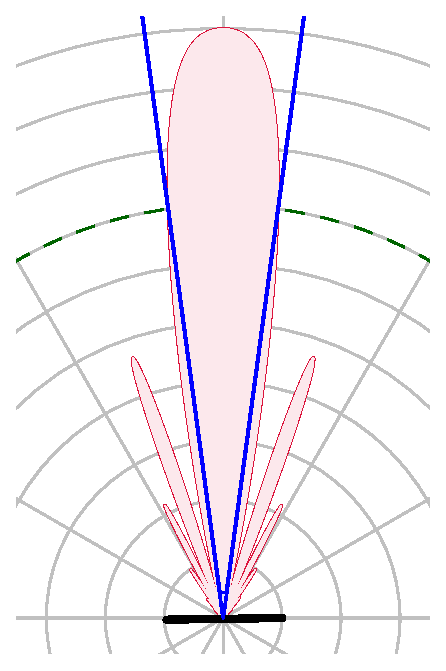
\includegraphics[scale=0.6,trim={0.46 0.072 0.46
	1.03},clip]{Chap2/fig/directivity.eps}
	\caption{Farfield beam shape and its \textit{beamwidth} (in blue).}
	\label{fig:beamwidth}
\end{figure}

On the other hand, there are hydrophone arrays that can infer the sound
direction by relating the spacing between the transducers with the signal
difference received by each of them \cite{bearing}.




\subsection{Available Models}
\label{ss:avaible_models}
 
\cite{sonars:16} % tipos de sonar

\section{Simulation}

Works on \textit{computacional ocean
acoustics}, the subfield of knowledge that explores the algorithms that model
the ocean as an acoustic medium, are well documented by
\citet{Etter2013}. Most of these works focus on very long range simulations,
with its most important features been the ocean floor and sub-bottom region.

This work aim to reconstruct and simulate near-range partially closed
environments, as those created by humans. The motivation for such a choice comes
from hydroeletrict power plant water intake, it is a corridor-like environment
with possible obstacles on the bottom. This kind of envirnoment is not well
covered on the underwater acoustics literature, as such, some of the simulations
techniques are borrowed from the closelly related are of \textit{room acoustics}.

When constructing a simulation one has to consider the tradeoff between
simplicity/perfomance/accuracy. There are several possible techniques with
different applications and assumptions, this chapter will cover the most
relevant ones and further explore \textit{ray theory}, which has been used for
the simulation presented here.

\subsection{Techniques Overview}

The idea behind sound simulation techniques is to solve the wave
equation (eq. \ref{eq:wave}) considering all the physical interfaces as boundary
conditions. The equation, however, cannot be analitically solved due to common
present discontinuities caused by occlusions, specular highlights and other
facts that result in large variations of the field over small regions of the
domain of integration\cite{funkhouser2003survey}.

The single most important reason that differentiate the several approches
described here is the \textit{wave frequency}. For high-frequency (where sound
speed do not very much in a wavelength scale) geometric methods (ray theory) are
justifiable and preferable (in the computational sense) \cite{urick1979}. In the
case of low/mid - frequency or in the presence of caustics\footnote{A region of
high constructive interference that geometrically gives a point of infinity
rays convegence.} other wave methods (e.g. finite elements, normal modes,
parabolic approximation) should be applied.

Instead of using the full wave equation, the methods work with a simplified
time-independ version. It starts by assuming that the equation
\ref{eq:wave}:

\[ \nabla^2 p - \frac{1}{c^2_0}\frac{\partial^2}{\partial t^2} p = 0 \]

Has a solution on the format:

\[ p(x,t) = a(x)\vartheta(t) \]

So that:
\[ \frac{\partial}{\partial t}a = 0 \]
\[ \nabla^2 \vartheta = 0 \]

Substituting it back and rearanging terms, gives:

\[ \frac{\nabla^2 a}{a} = \frac{1}{c_0^2\vartheta} \frac{\partial^2}{\partial
t^2}\vartheta  \]

As the expressions on both sides vary indepently, ie. l.h.s. varies with space
$s$ and r.h.s. with time $t$, they must be constant. As a matter of ajusting the
equation to fit its stantard parametrization, this constant is chosen to be
$-k^2$, then:

\[ \frac{\nabla^2 a}{a} = -k^2  \]
\[ \frac{1}{c_0^2\vartheta} \frac{d^2}{dt^2}\vartheta = -k^2  \]

Or

\begin{equation}
\label{eq:helmholtz}
(\nabla^2 -k^2)a = 0 
\end{equation}

\[ (\frac{d^2}{dt^2} + (kc_0)^2)\vartheta = 0  \]

With the apropriate definition of $\omega \equiv kc_0 $ the last equation,
becomes:

\begin{equation}
(\frac{d^2}{dt^2} + \omega^2)\vartheta = 0
\end{equation}

Equation \ref{eq:helmholtz} is known as the (homogeneous) \textit{Helmholtz
equation} and describe the time-independ part of the wave propagation. The
values of $k$ and $\omega$ can be phisically interpreted as the spatial and
tempral angular frequency of the wave. As the wave equation is a linear
equation superposition applies, it is resoanble to take into consideration
one wave frequency at a time and superpose all these harmonics by Fourier
synthesis\cite{Lefebvre}.



\subsubsection{FEM - Finite Element Method}\cite{funkhouser2003survey}
\subsubsection{Ray theory} \cite{torres2007modeling} \cite{danesh2013real}
\subsubsection{Normal modes} \cite{Etter2013}(?)
\subsubsection{Parabolic approximation} \cite{LURTON}

\subsection{Ray Theory}
\subsection{3D Enviroment Specifics}
\subsection{Results}

\section{Environment}

Extensive literature have been written on ocean environment, from modeling its
behaviour to measuring its properties. Different simulation techniques have also
been explored\cite{Etter2013}. The modeling presented here, althouth simple,
completely suits the needs of a ray tracing technique, presented on section
\ref{ss:raytheory}.

\subsection{Modeling}
\label{ss:modeling}
Borrowed from computer graphics, the modeling properties of a scene objectes
are the same for light and sound (given the high frequency limit for which ray
theory is applicable). Two distinct factors are modeled, one is geometric,
which defines the shape of the object, the other is acoustic, expressing how
does it interact with sound.

For the geometric part, two basic functions have to be provided: \textbf{intersection}
and \textbf{normal}. \textbf{Intersection} takes a ray, defined by a origin point and a
direction, and outputs the distance to the first intersection point with the
object. If no intersection point is found, the distance is defined to be
infinity. \textbf{Normal} receives a point on the surface of the object and
return the normal vector at such a point. Algorithm \ref{alg:rectangle}
exemplifies the \textbf{intersection} for a rectangle, the rays origin
$\mathbf{O}$ and direction $\mathbf{D}$ are matrix with the concatenated
information of all those whose intersection ought to be calculated.

\begin{algorithm}
\caption{Intersection for Rectangle}
\label{alg:rectangle}
\begin{algorithmic}
\Function{Intersection}{$\mathbf{O},\mathbf{D}$}\Comment{$\mathbf{O}$
is ray origin, $\mathbf{D}$ is direction} 

\State $\Delta \gets center -
\mathbf{O}$ \Comment{$center$ is the rectangle center}

\State $n \gets \nicefrac{\vec{s_1} \times  \vec{s_1}}{\norm{\vec{s_1} \times  \vec{s_1}}}$
\Comment{$\vec{s_1}$ and $\vec{s_1}$ are the rectangle's half-sides} 
\State $T \gets \left[ \vec{s_0} ~ \vec{s_1} \right]^\dagger$
\Comment{$^\dagger$ is pseudoinverse}
\State $d \gets \nicefrac{\Delta \cdot n}{\mathbf{D} \cdot n}$
\Comment{distance to intersection point}
\State $P \gets \mathbf{D}d - \Delta$
\Comment{$P$ are the intersection with the rectangle's plane}
\State $R \gets T \cdot P$
\Comment{$R$ are the intersection described on $\left[ \vec{s_0} ~ \vec{s_1}
\right]$ basis}

\ForAll{$i \in \left[0,\ldots,\text{size}(d)\right)$}
\If {$d_i < 0$ or $|R_{i,0}|>1$ or $|R_{i,1}|>1$}
\State $d_i \gets \infty$
\Comment{Check ray direction and if hit within rectangle}
\EndIf  
\EndFor


\State \textbf{return} $d$

\EndFunction
\end{algorithmic}
\end{algorithm}

Any surface can be approximated by triagulation and have these functions more
easily defined, but it is interesting to directly define for some geometric
primitives. Plane, rectangle, sphere and cylinder were developed for this work.

Two environments were constructed using these four geometric primitives. One
box-like for the reconstruction part of this thesis, which is simple enough to
study the properties of the mapping. Another, more complex and inspired on a
water entrance of a hydroeletric powerplant, that exibits a richer sonar
response with sound multipath and directional gain playing a more imporntant
role.

For the \textbf{box-like structure}, five planes were used thus determining a
semi-infinite box with 8 meters width, 10 meters length and the bottom 3 meters
from the origin. All planes are defined by a point and its normal vector.

\begin{table}[ht]
\centering
\begin{tabular}{lcc}
Plane Number & Point & Normal Vector \\
\hline
0 & $( 0, 4, 0)$ & $( 0,-1, 0)$  \\
1 & $( 0,-4, 0)$ & $( 0, 1, 0)$  \\
2 & $( 5, 0, 0)$ & $(-1, 0, 0)$  \\
3 & $(-5, 0, 0)$ & $( 1, 0, 0)$  \\
4 & $( 0, 0,-3)$ & $( 0, 0, 1)$  \\
\end{tabular}
\caption{Five planes defining box-like environment walls.}
\end{table}

The more \textbf{complex scene} is composed of 5 rectangles, 2 planes and a sphere
representing, respectively, 5 contrete walls, river floor and still surface
water and a half-spherical montain of sediments. Rectangles are defined by a
central point and two perpendicular vectors, the half sides, and spheres by a
center and radius.

\subsection{Characterization}
\label{ss:characterization}

Instead of defining a full BRDF (explained on section
\ref{sss:rays}), three parameters are considered: \textbf{diffusion coefficient},
\textbf{specular coefficient} and \textbf{shininess}. All three parameters may
change at every point on the surface of an object, thus defining a texture, but
for the sake of simplicity only constant values over the surface were
considered.

The \textbf{diffusion coefficient} and \textbf{specular coefficient} are,
respectively, fractions of incident energy over a surface patch that reflects
diffusely (as a lambertian reflector) and specularly. Reflections near
specularity are weighed as Phong reflection for a less unrealiscaly abrupt
change in reflection intensity. The \textbf{shininess} is the Phong parameter.
These concepts are described in section \ref{sss:rays}.

The actual values used came from a collection of sources in addition to
experimentation and tacit knowledge (from previous sonar use), as these are
difficult information to find in the literature.

For concrete, \citet{chirp} studies the \textbf{reflection coefficient}, sum of
\textbf{diffusion coefficient} and \textbf{specular coefficient}, to
characterize the concrete's quality following earlier measurements of
\citet{leslie1949ultrasonic}. The table provided on the article can be used in
the other direction, to simulate such a concrete quality. The individual values of \textbf{diffusion coefficient} and \textbf{specular coefficient} still
have to be determined and come from a educated guess based on considerations of
smooth by \citet{Etter2013}, which claims that most of the energy goes as
specular reflection for smooth surfaces. For
simulation purposes it has been consided values between 80\% to 95\% of the reflected energy to be specular.

\begin{table}[ht]
\centering
\begin{tabular}{rc}
Quality Of Concrete & Reflection Coefficient \\
\hline
Very good & $0.76$ or above  \\
Good & $0.69$-$0.74$  \\
Questionable & $0.62$-$0.69$  \\
Poor & $0.48$-$0.62$  \\
Very Poor & $0.48$ or less  \\
\end{tabular}
\caption{Quality of Concrete and Reflection Coefficient.
(\citet{chirp,leslie1949ultrasonic})}
\end{table}

\citet{Etter2013}, also, provides equations relating wind speed with water
surface reflection coeffiecient, which varies according to its roughness caused
by the wind. For a still water there is amost no transmitted energy and all
reflected energy is specular. For other materials, estimated values come from
models as the one provided by \citet{miller2015real} on
figure\ref{fig:materials}.

\begin{figure}[h]
	\centering
	\includegraphics[width=0.8\textwidth]{Chap2/fig/materials}
	\caption{Materials reflective characteristics from \citet{miller2015real}.}
	\label{fig:materials}
\end{figure}


%\subsection{3D Enviroment Specifics}
\section{Implementation}

\subsection{Algorithm}
\label{ss:algorithm}

The simulation follows the ray tracing technique outlined by
~\citet{bell1997simulation} for side scan sonar, but applies it to a forward
looking sonar imaging sonar (Section \ref{ss:avaible_models}). It also uses a
noising adding step as suggested by~\citet{coiras2009gpu} with statistics
provided by~\citet{maussang2007mean}.
No movement induced distortion was considered, some approaches to add this
feature is available in~\citet{bell1999techniques,borawski2005sonar}. Also,
spreading and absorption losses are ignored, assuming they are compensated by
TVG (see Section \ref{sss:tvg}).

Sonar parameters follow a Tritech's Micron sonar~\cite{micronsonar}
information as output power, dynamic gain, beam step and sensibility were found
on official Tritech's documentation~\cite{micronsonar,micronmodem}. The directional
gain was measured by the National Physical Laboratory, UK.

Simulation's output is, just as on the sonar, a sequence of arrays with values
between 0 and 255. Each element of the sequence is a bearing, direction of the
emitted sound pulse, and the array's components are the bins' values, sound
intensity received at some range of distances (calculated from echo delay).

\begin{figure}[h]
	\centering
	\includegraphics[scale=1.,clip]{Chap2/fig/sonarresponse.eps}
	\caption{Example of an array for a bearing direction. Actual arrays are
	longer, depending on resolution.}
	\label{fig:bins}
\end{figure}

The algorithm implementation uses the programming language Python with the
mathematical library NumPy, specially for efficient linear algebra. Most of the
treatment uses linear algebra to treat batch of rays at once.

\begin{figure}[ht]
    \centering
    \subfloat[Sonar Loop]{{\includegraphics[width=65mm]{Chap2/fig/sonarflow}}}%
    \hfill
    \subfloat[RayTracer]{{\includegraphics[width=85mm]{Chap2/fig/raytraceflow}}}%
    \caption{Overview of the simulation algorithm.}%
    \label{fig:algorithm}%
\end{figure}

Flowchart of Figure \ref{fig:algorithm} describes the simulator logic. It starts
by computing ray directions spread over a sphere centered at the sonar with
uniform density, otherwise it would bias the ray trace. Not all directions are
actually computed because some directions have very low gain, so rays in these directions
have almost no energy, they can be discarded. To compute such a uniformly
distributed directions apply transformation described by algorithm
\ref{alg:urays} for $[-\alpha,\alpha]$ and $[-\beta,\beta]$ the vertical and
horizontal angular span, respectively, and $N$ the desired number of rays.
Results in Section \ref{ss:results} use $\alpha = 30^o$ and $\beta = 3^o$,
approximatly the values for which Micron cannot detect the echo. 


\begin{algorithm}
\caption{Rays Uniform Direction}
\label{alg:urays}
\begin{algorithmic}
\Procedure{Uniform Direction}{$\alpha,\beta,N$}

\State $\dif\theta \gets 2\cos(\nicefrac{\pi}{2}-\alpha)$
\State $\dif\phi \gets 2\beta $
\State $\rho \gets \sqrt{\frac{N}{\dif\phi\cdot\dif\theta}}$ \Comment{Estimated
density}
\State $N_\theta \gets \lceil\rho\cdot\dif\theta\rceil$
\State $N_\phi \gets \lceil\rho\cdot\dif\phi\rceil$
\Comment{$U(\coord{x})$ generates $\coord{x}$ uniform samples over $[0,1]$}
\State $\theta \gets \arccos(\dif\theta\cdot (2U(N_\theta)-1))$ 
\State $\phi \gets \dif\phi\cdot (2U(N_\phi)-1)$

\ForAll{$(\theta_i,\phi_i) \in \theta\times\phi$}
\State $x_i \gets \sin(\theta_i)\cos(\phi_i)$
\State $y_i \gets \sin(\theta_i)\sin(\phi_i)$
\State $z_i \gets \cos(\theta_i)$
\State $v_i \gets (x_i,y_i,z_i)$
\EndFor

\State \textbf{return} $v$
\EndProcedure
\end{algorithmic}
\end{algorithm}

The sonar bearing pace is adjustable and, following Tritech's Micron
configuration, it was set to $1.8^o$, thus, doing a complete scan on $200$ steps. For each step, ray
directions are changed (by a rotation) to match new bearing. Received gain is
calculated w.r.t. the front direction (bearing), as the bearing changes the gain
is automatically updated. Rays always carry 2 information: its actual
intensity (disregarding distance traveled decay) and its total traveled length.

A new bearing position invoke ray tracer algorithm. It begins by calling
the \textbf{intersection} function (described in Section \ref{ss:modeling}) for
each object in the scene, passing all rays as argument. Then it loops again on every
object, but now only focus on the rays that have the object as first hit, and
compute the backscattering to the sonar. Backscattering strength calculation use
Lambert and Phong scatterings as described in Section \ref{sss:rays} and material
parameters listed in Section \ref{ss:characterization}. This strength is addad
to a bin (see Figure \ref{fig:bins}) whose position is calculated as half the full
distance traveled by the ray (including previous reflections) plus a small
gaussian noise. It proceeds to calculate reflection if the number of computed
reflection for the ray does not exceed a maximum value (set to 5). Reflections
are simple linear transformations that depends on the surface's normal, obtained
via \textbf{normal} function (Section \ref{ss:modeling}). The algorithm, then,
calls itself for the reflected rays, recursively.

\begin{figure}
	\centering
	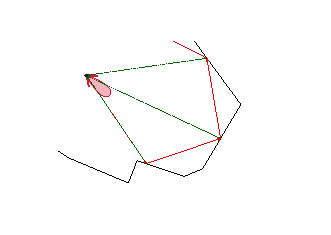
\includegraphics[scale=2.5, trim={20 20 20 20}, clip]{Chap2/fig/method.pdf}
	\caption{Ray Tracing: Red lines are specular reflections, green lines are diffuse backscattering.}
	\label{fig:methodtrace}
\end{figure}

After the whole scan is computed, bin values are normalized to $[0,\ldots,255]$
(again according to Tritech's Micron configuration ). Upon these values, an
additional Weibull's distributed noise is applied~\cite{maussang2007mean}.

\subsection{Results}
\label{ss:results}

For both environments described in Section \ref{ss:modeling}, several sonar
positions were simulated. The absolute position and orientation were chosen, but
the bearing w.r.t. the environment was a random value.

Polar plots displayed here is the expected visualization, without noise
filtering, when the sonar uses 500 bins of resolution with a 12 meters range.
Each polar pixel has a $3^o$ arc length, but, as the bearing step is $1.8^o$,
they overlap while being rendered.

\subsubsection{Box-like Environment}
The half-infinity box-like structure is depicted on figure
\ref{fig:box_simul}. Axis aligned sonar orientation on figures
\ref{fig:box_axis_center} and \ref{fig:box_axis_offcenter} make clear its
rectangular cross section, while its half-infinity characteristic is visible on
perpendicular oriented scans, figures \ref{fig:box_perp_center} and
\ref{fig:box_perp_offcenter}.


\begin{figure}[ht]
    \centering \subfloat[Position $(0,0,0)$ | Orientation
    $(1,0,0)$]{{\label{fig:box_perp_center}\includegraphics[width=75mm]{Chap2/fig/main_script__4_13_57_42_0,0,0_1,0,0f2}}}%
    \hfill \subfloat[Position $(4,1,0)$ | Orientation
    $(0,1,0)$]{{\label{fig:box_perp_offcenter}\includegraphics[width=75mm]{Chap2/fig/main_script__4_14_12_04_4,1,0_0,1,0f2}}}%
    \\
    \subfloat[Position $(0,0,0)$ | Orientation
    $(0,0,1)$]{{\label{fig:box_axis_center}\includegraphics[width=75mm]{Chap2/fig/main_script__4_14_14_06_0,0,0_0,0,1f2}}}%
    \hfill \subfloat[Position $(0,3,0)$ | Orientation
    $(0,0,1)$]{{\label{fig:box_axis_offcenter}\includegraphics[width=75mm]{Chap2/fig/main_script__4_14_18_20_0,3,0_0,0,1f2}}}%
    \caption{Sonar simulation for the box-like scene.}%
    \label{fig:box_simul}%
\end{figure}

\subsubsection{Complex Environment}

Figure \ref{fig:jirau_simul} shows the more complex structure from four view
points. Images \ref{fig:complex_inner_mid} and \ref{fig:complex_inner_low} are scans from between walls of the indent. Figure
\ref{fig:complex_out_mid} is cross sectional view of the indent and figure
\ref{fig:complex_out_low} is a scan from the same position, but with different
orientation, making the hemisphere at the bottom more noticeable.

\begin{figure}[ht]
    \centering \subfloat[Position $(0,0,0)$ | Orientation
    $(1,0,0)$]{{\label{fig:complex_inner_mid}\includegraphics[width=75mm]{Chap2/fig/main_script__4_02_09_57_0,0,0_1,0,0f2}}}%
    \hfill \subfloat[Position $(0,0,6)$ | Orientation
    $(1,0,0)$]{{\label{fig:complex_inner_low}\includegraphics[width=75mm]{Chap2/fig/main_script__4_02_10_19_0,0,6_1,0,0f2}}}%
    \\
    \subfloat[Position $(-5,0,12)$ | Orientation
    $(0,1,0)$]{{\label{fig:complex_out_low}\includegraphics[width=75mm]{Chap2/fig/main_script__4_02_16_13_-5,0,12_0,1,0f2}}}%
    \hfill \subfloat[Position $(-5,0,12)$ | Orientation
    $(0,0,1)$]{{\label{fig:complex_out_mid}\includegraphics[width=75mm]{Chap2/fig/main_script__4_02_21_25_-5,0,12_0,0,1f2}}}%
    \caption{Sonar simulation for the complex scene.}%
    \label{fig:jirau_simul}%
\end{figure}

Both environemnts reveal interesting features of a sonar scan, but they tend to
be more pronounced on the complex environmnt. Figures
\ref{fig:complex_inner_low}, \ref{fig:complex_out_mid} and
\ref{fig:box_perp_offcenter} present clear signal of multipath. Another
interesting feature is the halo on the background of figures
\ref{fig:complex_inner_mid} and \ref{fig:complex_inner_low} caused by a
trade-off between the sonar directional gain and the low backscattering at
shallow angles.
